% !TEX TS-program = pdflatex
% !TEX encoding = UTF-8 Unicode


\documentclass[11pt]{article}
\usepackage[utf8]{inputenc}

%%% PAGE DIMENSIONS
\usepackage{geometry}
\geometry{letterpaper}
\geometry{margin=1in} % for example, change the margins to 2 inches all round

\usepackage{graphicx} % support the \includegraphics command and options
\usepackage[parfill]{parskip} % Activate to begin paragraphs with an empty line rather than an indent

%%% HEADERS & FOOTERS
\usepackage{fancyhdr} % This should be set AFTER setting up the page geometry
\pagestyle{fancy} % options: empty , plain , fancy
\renewcommand{\headrulewidth}{0pt} % customise the layout...
\lhead{}\chead{}\rhead{}
\lfoot{}\cfoot{\thepage}\rfoot{}

%%% SECTION TITLE APPEARANCE
\usepackage{sectsty}
\allsectionsfont{\sffamily\mdseries\upshape}
% (See the fntguide.pdf for font help)
% (This matches ConTeXt defaults)

%%% END Article customizations

\title{Slow Earthquakes: A Manifestation of Transitional Frictional Behavior}
\author{J.R. Leeman, D.M. Saffer, C. Marone}
\date{} % Activate to display a given date or no date (if empty),
         % otherwise the current date is printed

\bibliographystyle{unsrt}

\begin{document}
\maketitle

\section{Introduction}
Observations of slow-slip and low-frequency earthquakes in nature suggest that
fault failure encompasses a spectrum of slip modes \cite{Peng:2010, Ide:2007,
Beroza:2011}.  While the explanations for non-traditional earthquakes remain a
topic of debate, they have been observed in many subduction zones, including
Cascadia \cite{Miller:2002, Rogers:2003}, Mexico \cite{Kostoglodov:2003}, Costa
Rica \cite{Jiang:2012}, Japan \cite{Ito:2006}, and New Zealand
\cite{Wallace:2010}. What causes strain energy to be released across a
wide-range of failure behaviors is not well understood, but transitional
frictional stability is a  possible explanation. System stability is defined in
terms of system stiffness ($k$) related to the critical stiffness ($k_{c}$) \cite{Gu:1984} and can be altered by
environmental variables such as effective normal stress, critical slip distance,
and the velocity dependence of friction. Clustering of slow and transitional
events around traditional seismic faults in nature suggests that transitional
behavior is responsible. Laboratory evidence of this behavior is scattered
\cite{Kaproth:2013, Baumberger:1994, Leeman:2015}, mostly suggested by numerical
models \cite{Gu:1984}. Here we present the first systematic investigation of the
critical stiffness ratio and its effect on the frictional state of a laboratory
fault. We also show that stiffness can control the slip mode and that the
slip mode can change as stiffness is influenced by accumulated fault slip and
damage zone evolution.


\section{Main}

The observation of non-traditional slip modes (slow slip, very low frequency
earthquakes, episodic tremor and slip, etc) in a wide variety of locations
over the last decade suggests that this is a common occurrence. There have been
suggestions that these behaviors, often observed at the down-dip limit of
traditional seismic slip, can influence, interact with, or trigger up-dip
earthquakes \cite{Dragert:2001ed,Ide:2007fi}. There has also been the suggestion
that these events occur at the transition between stable and locked patches
of a fault and that non-traditional slip areas could influence earthquake
nucleation in those areas \cite{Linde:1996hn}.

The rate-and-state friction framework is commonly used to describe the dynamic
frictional behavior of natural and experimental systems to perturbations. This
empirical relation consists of the parameters $a$ and $b$ which describe the
velocity dependence of friction. For materials in which $(a-b)>0$ the friction
increases with increased driving velocity, termed velocity strengthening. Likewise,
materials with $(a-b)<0$ are velocity weakening. The model also consists of an
$e$-folding critical slip distance $D_c$, and a state variable $\theta$.
$D_c$ is thought of, in the laboratory, as the distance required to completely
renew a contact population.
The
state variable is thought to be a proxy for the age of the frictional contacts, and
evolves according to a state evolution relation, commonly the Dieterich `slowness'
or Runia `slip' relation \cite{Marone:1998,Dieterich:1979,Ruina:1983}.

For unstable behavior to occur: 1) that the material be
velocity neutral to velocity weakening, and 2) that the system stiffness be at
or below the critical stiffness \cite{Marone:1998, Scholz:2002}. If a
material is velocity strengthening, any acceleration leading to slip is
immediately arrested by increased shearing resistance and the energy is
frictionally dissipated. The stiffness of the system governs the rate at which
energy stored as strain can be released. If the energy release occurs in such a
way that the drop in shear resistance with displacement occurs faster than the
drop in applied shearing force with displacement, the system can support
unstable failure. The critical stiffness can be described in terms of the
rate-and-state parameters as (eq.\ref{equation:kc}). The aggregate stiffness of
the loading system and sample can be measured by fitting the linear-slope
of the load-point displacement vs. shear load curve on either an unload/reload
cycle or on the loading portion of a single stick-slip event \cite{Leeman:2015}.

% Equation - Critical Stiffness %
\begin{equation}
    K_c = \sigma_n' \frac{b-a}{D_c}
    \label{equation:kc}
\end{equation}
% End Equation %

We conducted a suite of biaxial double-direct shearing experiments with a fine
quartz fault gouge simulant (Min-U-Sil\textsuperscript{\textregistered}), chosen
for its geologic relevance, reproducible results, and well controlled
composition and size distribution. This study systematically examines the
behavior of an experimental fault as a function of nearness to the stability
criterion $k \sim k_c$. Using the same, well  controlled sample material for
each experiment and humidifying the samples, we ensure that the rate-and-state
parameters $(a,b,D_c)$ remain essentially constant between experiments. We then explore the stability
of the system by modifying the stiffness directly by changing the forcing block
configuration and by changing the applied effective normal stress $(\sigma_n')$.

% Figure %
\begin{figure}
    \centering
    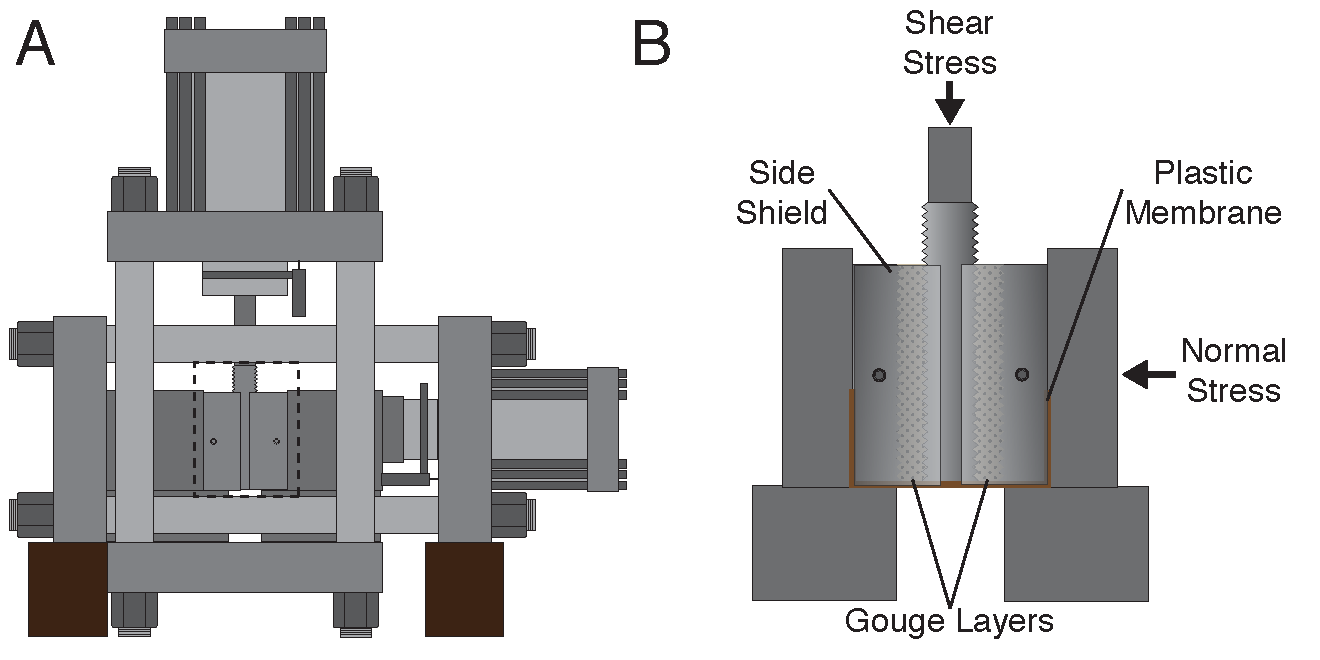
\includegraphics[scale=0.5]{../Figures/Fig_Biax_Schematic/biax_schematic.pdf}
       \caption{The biaxial deformation apparatus (A) and sample configuration (B).
       Two large hydraulic pistons are servo-controlled in either force or
       displacement control modes. Double direct shear samples are supported by
       steel blocks. Samples use metal side shields and a plastic membrane to
       reduce gouge extrusion.  Local displacement transducers (DCDTs) can be
       referenced to the center block to avoid apparatus stiffness effects on
       the measurement.}
      \label{Fig:Biax Schematic}
\end{figure}
% End Figure %

In order to define/measure the RSF parameters for each experiment, we use a
range of measurements. For experiments in which $K$ is high, stable sliding
behavior is  observed and we use velocity steps to obtain the rate-and-state
frictional parameters and therefore $K_c$.  We assume that the evolution of
these material and layer properties is not dependent on the mode of slip, and
therefore we use the values measured on stably sliding experiments as a
framework for evaluating/comparing results from the suite of experiments.


\section{Results/Discussion}

Our results show that the mode of slip is consistent with that expected from the
rate-and-state friction framework. Slip mode varies systematically with $K$,
and transitional behavior is observed at $\frac{K}{K_c} \sim 1$. In a stiff (all
steel) forcing setup, linearly stable behavior was observed, while in a
more compliant loading system, emergent unstable behavior was observed. Unstable
behavior began with frictional oscillations, transitionally to dynamic frictional
failure. Oscillations and dynamic failure are characterized by relatively rapid
accelerations and decelerations of the system above/below the load point
velocity when the material yields under excessive shear force. In experiments with
further increased compliance, rapid dynamic failure was observed. These events
were audible and classified as fast stick-slip.

We also observe that there is a relation between the peak velocity or duration
of slip and $\frac{K}{K_c}$. Systems near the stability transition exhibit
lower peak velocities and long duration events, seen as frictional oscillations
in the experiments. The further the system is from the transition, the events
become shorter in duration and faster.

Both $K$ and $K_c$, and thus mode of slip, evolve with net slip. As layer
accumulates strain and strain is localized, it stiffens. At the same time, RSF
parameters evolve, modifying the critical stiffness of the system. This explains
a rich variety of behaviors that may appear unrelated or non-linear initially.
This is supported by our observations that stick slip does not occur until a
critical displacement is reached, because $K_c$ is negative until the onset of rate
weakening behavior. Most stiffness evolution occurs in the first 10 mm of shear,
asymptotically approaching stead-state. Initial increases in stiffness could be
due to layer compaction from grain rearrangement, layer thinning with increased
shear strain, grain comminution, localization of shear, or reduction of
compliant center block material above the sample due to geometric effects. Layer
compaction due to rearrangement and geometric thinning with shear have been well
documented \cite{Scott:1994}.  At these low stresses, grain comminution is
minimal. Shear localization effects have been shown to play a role in the
evolution of layer behavior \cite{Logan:1992}, especially before reaching
mechanical steady-state as R and Y shears develop. The reduction in the amount
of compliant center block material above the shearing zone with accumulated
displacement is minimal compared to these other effects.

In our experiments, $a$ remains relatively constant with displacement, but $b$
evolves asymptotically upwards with increasing shear displacement. During this
transitional period, the critical slip distance evolves downwards
(Fig.\ref{Figure:RSF Props}).

% Figure %
\begin{figure}
    \centering
        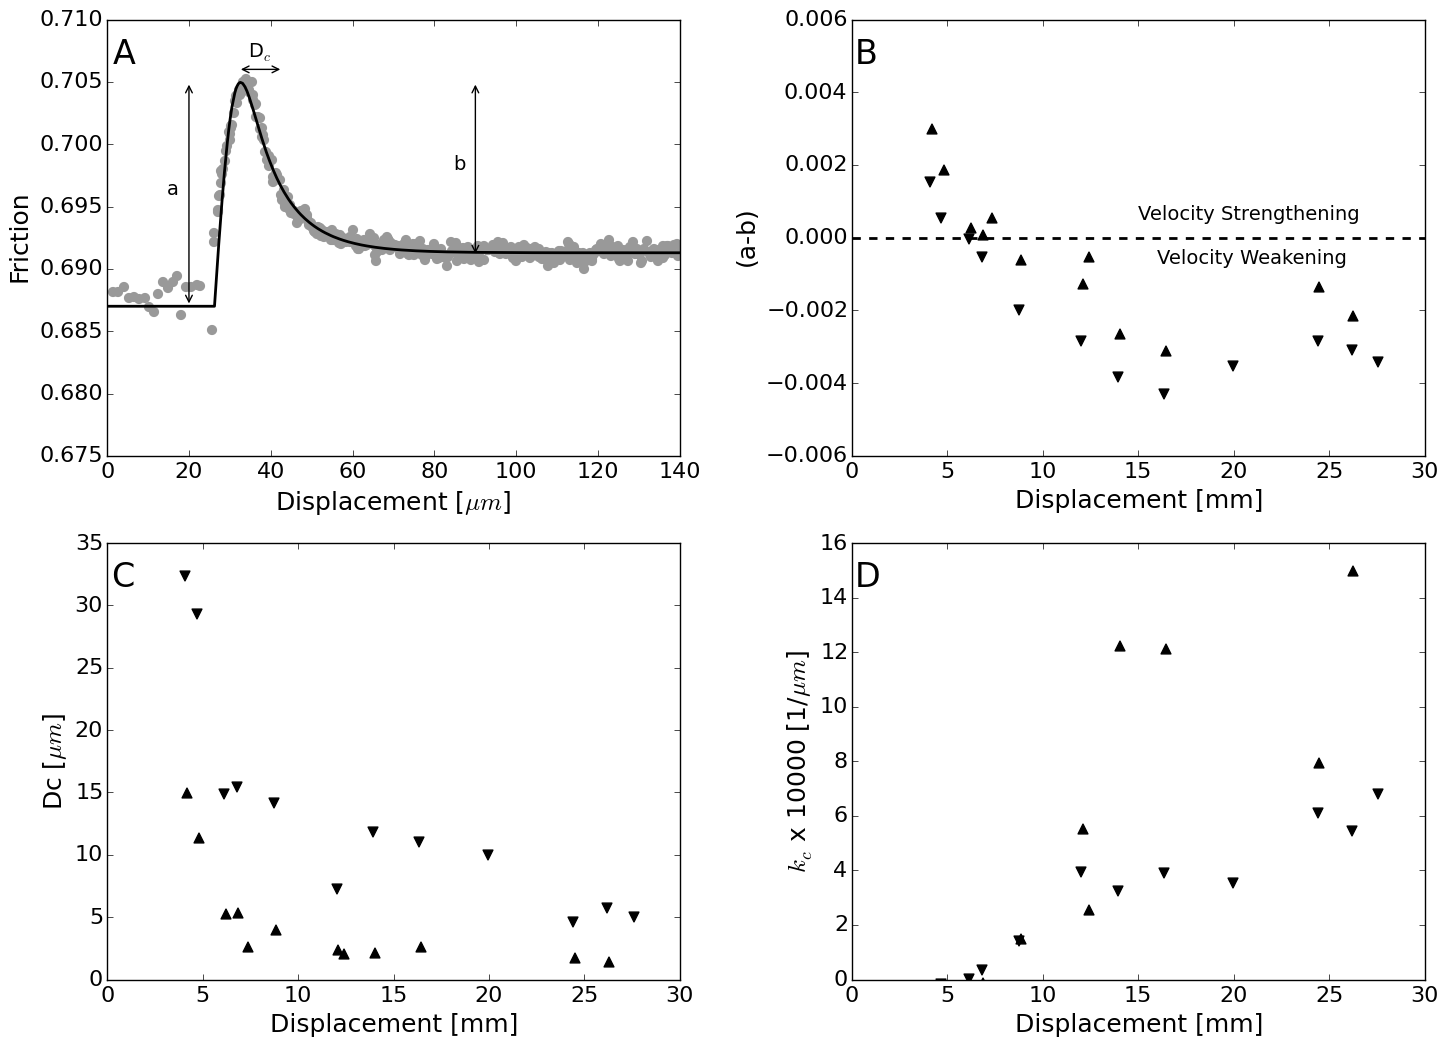
\includegraphics[scale=0.45]{../Figures/Fig_RSF_Parameters/RSF_Parameters.png}
       \caption{Rate-and-state friction parameters obtained from velocity step
       inversions. All inversions were accomplished with a fixed stiffness of
       $k=$5.5x$10 ^ {-3} \mu$m. A) rate-and-state parameter $a$ remains relatively
       constant with displacement and shows a systematic behavior with higher
       values of $a$ always being observed during velocity up-steps. The $b$
       parameter shows a similar behavior, but also increases with displacement,
       reaching a steady-state value $\sim$10 mm displacement. B) The sample
       transitions from velocity strengthening to velocity weakening  behavior
       at $\sim$10 mm and remains velocity weakening for the remainder of  the
       experiment. C) Critical slip distance estimates show considerable
       scatter,  but do reduce to a steady-state value of 5-10 um.}
      \label{Figure:RSF Props}
\end{figure}
% End Figure %

% Figure %
\begin{figure}
	\centering
		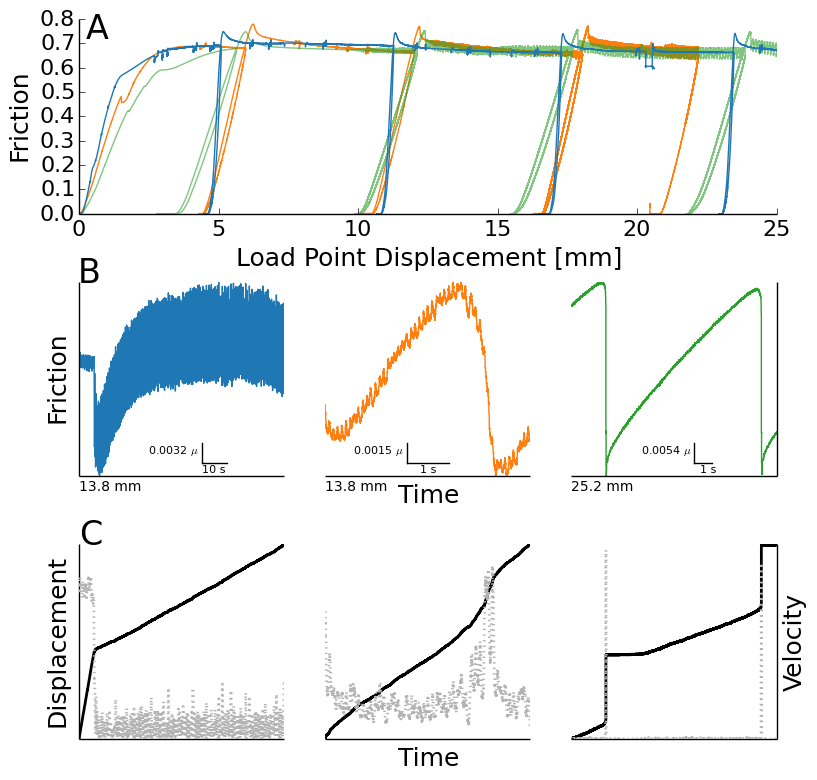
\includegraphics[scale=0.7]{../Figures/Fig_Runplot/runplot.png}
   	\caption{A) Run-plots of experiments p4309 (blue), p4311 (orange), and p4316
   	(green). Different working stiffnesses can be observed as the slope of
   	unload/reload segments. B) All steel blocks produced stable responses to
   	velocity steps (left). Destiffening the system with an acrylic center block
   	produced non-audible slow-slip events (center). Further destiffening with an
   	acrylic center block and increased normal stress produced audible fast
   	stick-slip events(right). C) Center block displacement (black) and velocity
   	(gray) for the corresponding types of failure.}
  	\label{Figure:Runplot}
\end{figure}
% End Figure %

Our results support previous ideas about the role of transitional frictional
properties in supporting a range of complex failure behaviors. Natural factors
such as compliant and evolving damage zones, low effective normal stress
\cite{audet2009seismic,kitajima2012elevated,shelly2015complexity},
and fault evolution/aging \cite{ikari2011relation} are all captured in the
simple ratio of $\frac{K}{K_c}$.  All of this
suggesting that tectonic faults may change behavior as they accumulate slip and
become mature fault zones.

% Figure %
\begin{figure}
    \centering
        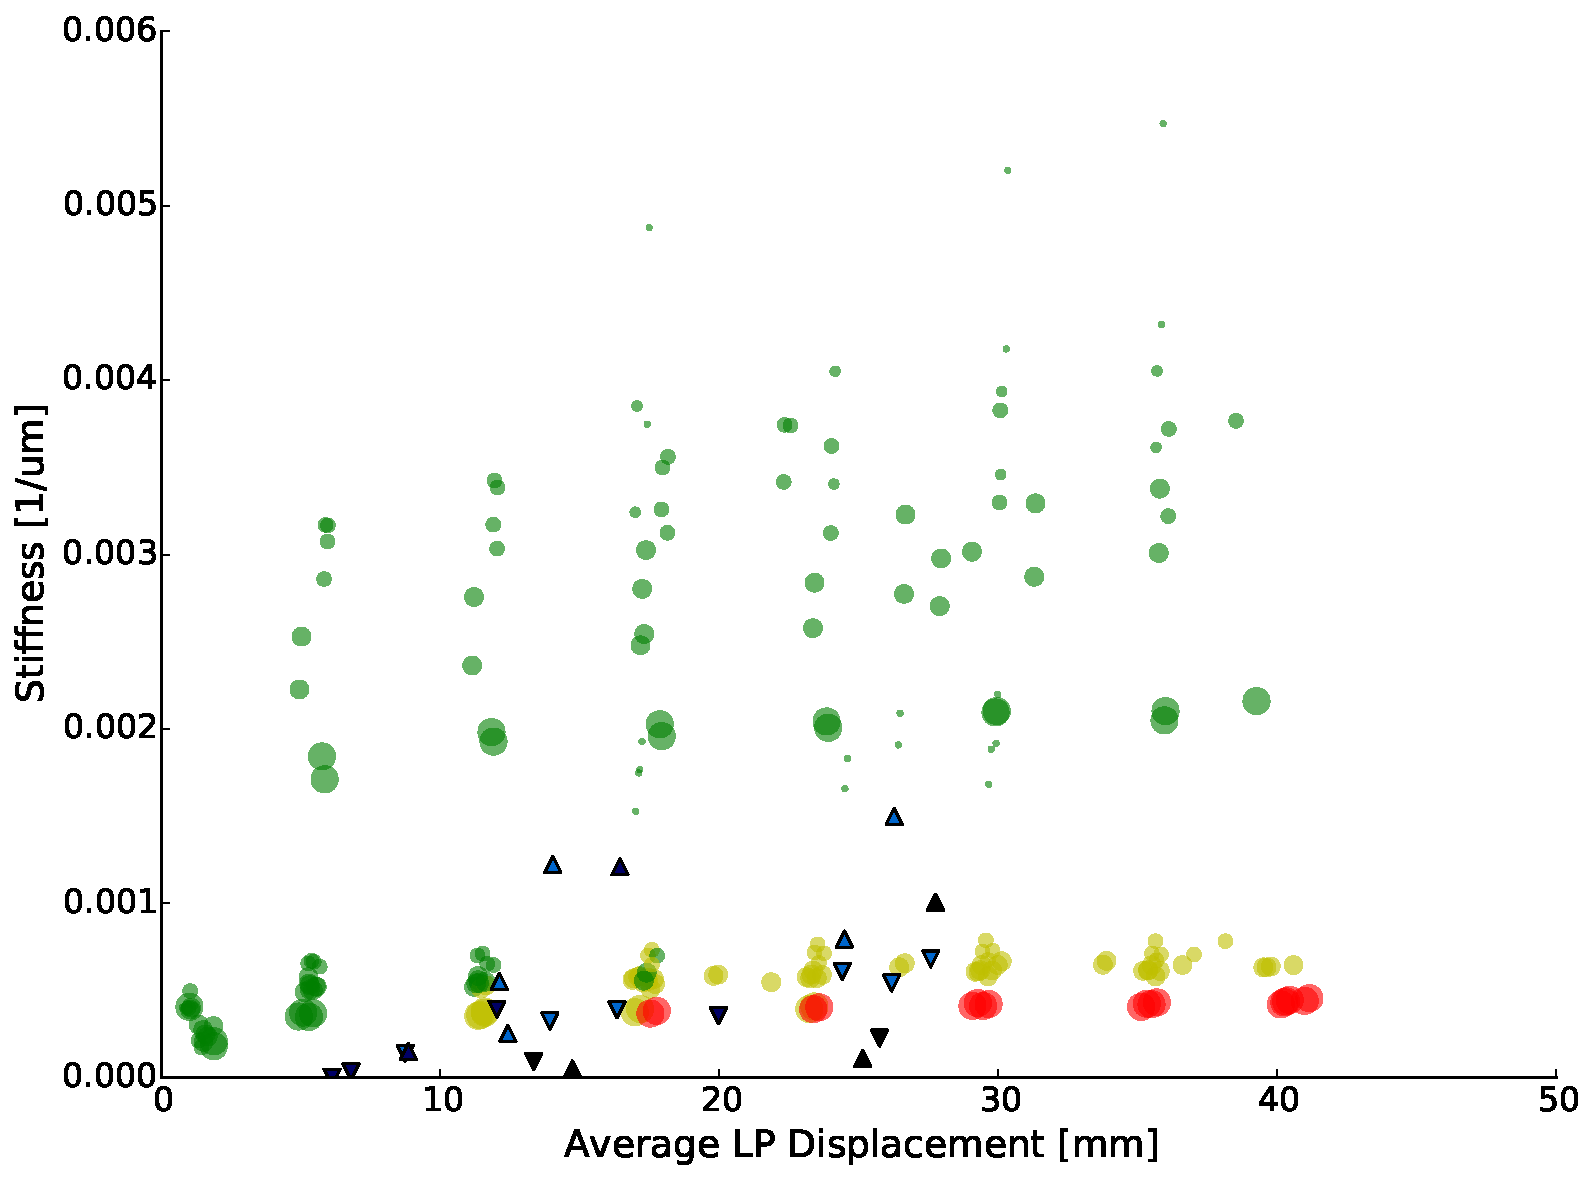
\includegraphics[scale=0.4]{../Figures/Fig_Stiffness_Evolution/Stiffness_Evolution.pdf}
       \caption{Stiffness estimates from shear stress unload/reload cycles show
       an increase in the stiffness early in shearing, likely associated with
       fabric development. Experiments with stiffness comparable to the critical stiffness
       estimates from velocity steps exhibit slow-slip behavior. Experiments in
       which the measured stiffness is below the critical stiffness exhibited
       more rapid, audible stick-slip.}
      \label{Figure:Stiffness Evolution}
\end{figure}
% End Figure %

With slow-slip failure events, we see little to no dynamic overshoot. This is observable by a period of no block motion or
deformation after the rapid stress-drop (Fig.\ref{Figure:Runplot}C).  In
traditional fast stick-slip events, the system shears further than required to
complete the force balance. Frictional oscillations and slow-slip
show no such overshoot, with continual deformation of the system throughout the
simulated seismic cycle. This provides some insight into the low frequency
nature of emissions observed from slow-slip and lack of audible report in the
laboratory. Lower shear stiffnesses will reduce the seed of rupture propagation,
softening step-like acceleration/deceleration pulses that result in high
frequency emission. Slowed rupture velocities would also influence disaster potential, as
tsunamogenic earthquake have generally slow rupture velocities
\cite{Kanamori:1993, Bilek:1999}.

We suggest that where in the spectrum of failure behavior a fault lies can be
quantitatively described by the relation of the stiffness of the fault compared
to the calculated critical stiffness. While factors such as pore pressure and
material frictional response are important, they are already factored into  the
stiffness comparison.

\section{Methods}
All experiments were performed on a servo-controlled biaxial shearing apparatus.
Displacements on the normal and shearing axes were measured by Direct Current
Displacement Transducers (DCDTs) referenced at the end-platens and ram nose. The
displacement of the shearing block was measured with a DCDT referenced at the
end-platen and the top of the shearing block. Loads applied to the sample were
measured with strain gauge load cells. All transducers are semi-annually
calibrated with traceable transfer standards.

Samples were prepared in the double-direct-shear geometry using steel or
titanium side blocks and steel or acrylic shearing blocks. All blocks were
grooved 0.8 mm deep at 1 mm spacing to reduce boundary effects \cite{Anthony:2005}. The sample area
was 10 x 10 cm and filled with Min-U-Sil to a thickness of 3 mm. Granular layers
were left in a sealed container overnight with a solution of anhydrous sodium
carbonate to humidify the samples.

After samples were loaded into the load frame, a constant normal stress was
applied and maintained by the servo system in a force feedback control mode.
Samples were allowed to compact and accommodate grain rearrangement before
shearing began. Shearing is conducted at a fixed rate in displacement feedback
control mode.

Stiffness of the system was altered by changing the applied normal stress and by
changing the material of the shearing block. Increasing normal stress decreases
the effective stiffness of the system, as does switching the steel forcing block
for a cast acrylic block.

Layers were built of Min-U-Sil\textsuperscript{\textregistered} 40 fine ground
silica from the U.S. Silica\textsuperscript{\textregistered} company Berkeley
Springs, West Virginia plant. The median diameter of grain is 10.5 $\mu m$. The
product is 99.5 \% SiO$_2$, with traces of metal oxides making up the remainder.

System stiffnesses from unload/reload shear stress cycles were calculated by a
least-squares linear fit in friction vs. displacement for the interval $\mu =
0.3-0.4$. Stiffnesses from the loading portion of slow-slip and stick-slip
events were obtained with a derivative based algorithm \cite{Leeman:2015}.
Rate-and-state models were fit with both the Dieterich and
Ruina laws, with comparable results. Inversions were done with an iterative
singular value decomposition technique.

\bibliography{references}

\section{Acknowledgements}
The authors wish to thank Steve Swavely for his support in the laboratory.
We also thank Marco Scuderi for many discussions regarding this work. This
material is based upon work supported by the National Science Foundation under
Grant No. DGE1255832.  Any opinions, findings, and conclusions or
recommendations expressed in this material are those of the author(s) and do not
necessarily reflect the views of the National Science Foundation. The work was
also supported by funds from the GDL Foundation and Shell Oil Company.

\section{Author Contributions}
All authors contributed to data interpretation, analysis schema, and writing.
J. Leeman conducted experiments and data analysis.

\section{Competing Financial Interests}
The authors declare no competing financial interests. Supplementary information
accompanies this paper on www.nature.com/naturegeoscience. Reprints and permissions information is
available online at http://npg.nature.com/reprintsandpermissions. Correspondence
and requests for materials should be addressed to J.R. Leeman.

\newpage
\section{Supplementary}

% Begin Table %
\small
\begin{center}
    \begin{tabular}{ | l l p{1.6cm} p{1.7cm} p{1.6cm} p{4cm} p{0.5cm} | }
\hline
Experiment & Blocks Used & Normal Stress [MPa] & Temperature [$^\circ$C] & Relative Humidity [\%] & Comments & Unload/Reloads \\
\hline
p4224      & Titanium/Acrylic & 5                   & 26              & 16                    & Stable - Velocity Steps         & N              \\
p4228      & Steel            & 4                   & 24              & 100                   & Stable - Slide Hold Slide       & N              \\
p4229      & Titanium/Acrylic & 4                   & 24              & 100                   & Failed Experiment               & N              \\
p4248      & Titanium/Acrylic & 4                   & 24.2            & 100                   & Stable - Velocity Steps         & N              \\
p4249      & Titanium/Acrylic & 4                   & 23.2            & 100                   & Stable - Velocity Steps         & N              \\
p4267      & Titanium/Acrylic & 2                   & 23.2            & 100                   & Stable - Velocity Steps         & Y              \\
p4268      & Titanium/Acrylic & 8                   & 23.4            & 100                   & Slow Slip                       & Y              \\
p4269      & Steel            & 4                   & 23.4            & 100                   & Stable - Velocity Steps         & Y              \\
p4270      & Steel            & 2                   &                 & 100                   & Stable - Velocity Steps         & Y              \\
p4271      & Titanium/Acrylic & 2                   &                 & 100                   & Stable - Velocity Steps         & Y              \\
p4272      & Titanium/Acrylic & 8                   & 22.7            & 100                   & Slow Slip                       & Y              \\
p4273      & Steel            & 8                   & 23.4            & 100                   & Stable - Velocity Steps         & Y              \\
p4309      & Steel            & 8                   & 23.2            & 100                   & Stable - Velocity Steps         & Y              \\
p4310      & Titanium/Acrylic & 8                   & 24.2            & 100                   & Slow Slip                       & Y              \\
p4311      & Titanium/Acrylic & 8                   & 23.3            & 100                   & Slow Slip                       & Y              \\
p4312      & Steel/Acrylic    & 8                   & 23.6            & 100                   & Slow Slip                       & Y              \\
p4313      & Titanium/Acrylic & 8                   & 23.5            & 100                   & Slow Slip                       & Y              \\
p4314      & Steel            & 12                  & 24.3            & 100                   & Stable - Velocity Steps         & Y              \\
p4316      & Titanium/Acrylic & 12                  & 23.6            & 100                   & Stick Slip                      & Y              \\
p4317      & Steel/Acrylic    & 12                  & 24.2            & 100                   & Stick Slip                      & Y              \\
p4327      & Steel            & 6                   & 22.5            & 100                   & Stable - Velocity Steps         & Y              \\
p4328      & Titanium/Acrylic & 6                   & 22.7            & 100                   & Slow Slip                       & Y              \\
p4329      & Titanium/Acrylic & 6                   & 22              & 100                   & Slow Slip                       & Y              \\
p4330      & Steel            & 6                   & 22.9            & 100                   & Stable - Velocity Steps         & Y              \\
p4338      & Titanium/Acrylic & 4                   & 24.2            & 100                   & Stable - Velocity Steps         & Y              \\
p4339      & Steel            & 4                   & 24.8            & 100                   & Stable - Velocity Steps         & Y              \\
p4340	     & Titanium/Acrylic & 8                   & 24.0            & 100                   & Slow Slip                       & Y              \\
p4341	     & Steel            & 12                  & 23.4            & 100                   & Stable - Velocity Steps         & Y              \\
p4342	     & Titanium/Acrylic & 12                  & 24.3            & 100                   & Slow/Fast Slip                  & N              \\
p4343	     & Steel/Acrylic    & 6                   & 23.9            & 100                   & Slow Slip                       & N              \\
p4344	     & Titanium/Acrylic & 7                   & 24.5            & 100                   & Slow Slip                       & N              \\
p4345	     & Steel/Acrylic    & 8                   & 24.2            & 100                   & Slow Slip                       & N              \\
p4346	     & Titanium/Acrylic & 9                   & 24.2            & 100                   & Slow Slip                       & N              \\
p4347	     & Steel/Acrylic    & 10                  & 23.1            & 100                   & Slow/Fast Slip                  & N              \\
p4348	     & Titanium/Acrylic & 11                  & 23.9            & 100                   & Slow/Fast Slip                  & N              \\
p4350	     & Steel/Acrylic    & 13                  & 22.7            & 100                   & Slow/Fast Slip                  & N              \\
p4351	     & Titanium/Acrylic & 14                  & 23.1            & 100                   & Slow/Fast Slip                  & N              \\


    \hline
    \end{tabular}
\end{center}
% End Table %


% Figure %
\begin{figure}
    \centering
        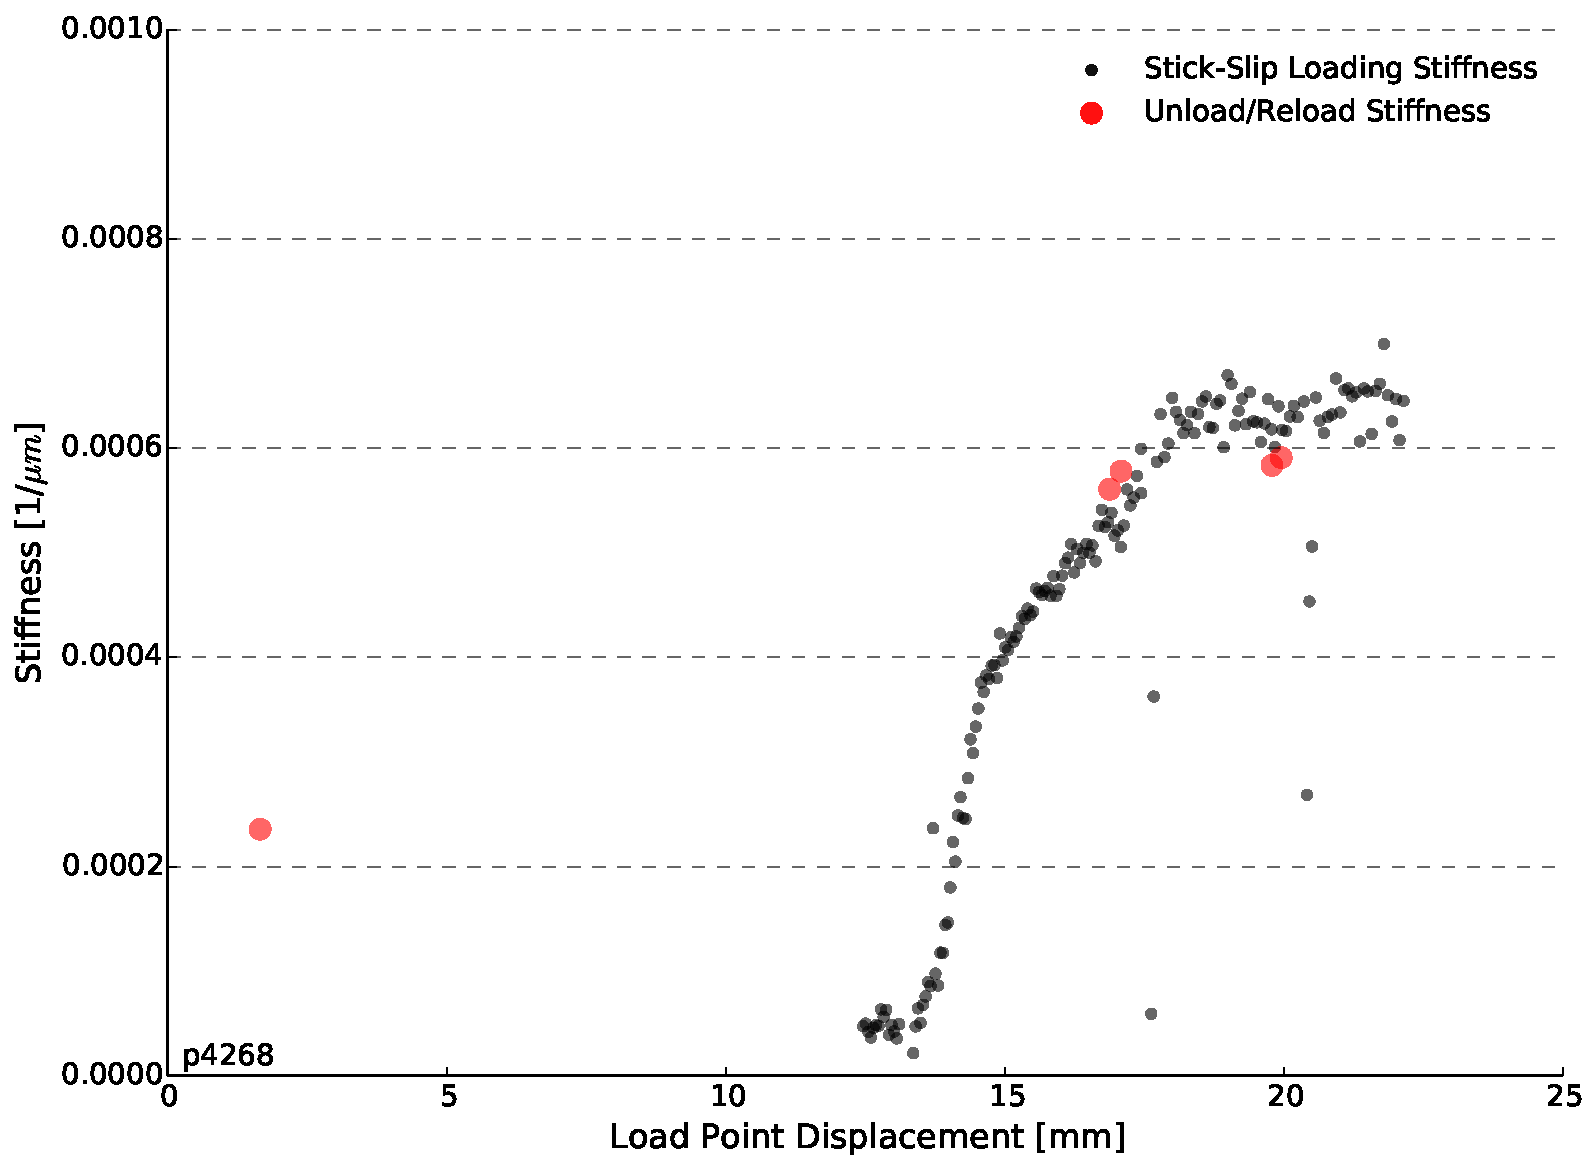
\includegraphics[scale=0.4]{../Figures/Fig_Stiffness_Methods/Stiffness_Methods.pdf}
       \caption{When the system is at steady-state, the two methods of stiffness
       estimation provide comparable results. At low displacements, early stick-slip
       events appear more compliant than bulk system measurements. This is due to the
       not fully dynamic failure of the events and creep during the loading phase.}
      \label{Figure:Stiffness Methods}
\end{figure}
% End Figure %


\end{document}
